%
% Sección de Introducción.
% Artículo.
% Proyecto Lovelace.
%

\section{Introducción}

% Contexto histórico: cómo llegó a ser popular la tokenización.

Cuando el comercio a través de Internet comenzó a popularizarse, los fraudes de
tarjetas bancarias se volvieron un problema alarmante: Visa y MasterCard
reportaron, entre 1988 y 1998, pérdidas de 750 millones de dólares; según
\cite{wallethub}, en el año 2001 se tuvieron pérdidas de 1.7 miles de millones
de dólares y, para 2002 aumentaron a 2.1. Como una medida para proteger los
sistemas procesadores de pagos, las principales compañías de tarjetas de crédito
publicaron un estándar obligatorio para todos aquellos que procesaran más de 20
000 transacciones anuales: el PCI DSS (en inglés, \textit{Payment Card Industry
Data Security Standard} \cite{pci_dss}).

El PCI DSS cuenta con una gran cantidad de requerimientos, entre ellos,
controles estrictos de acceso, monitoreo regular de redes, mantener programas de
vulnerabilidades y políticas de seguridad de información, etcétera
\cite{uk_association} \cite{search_security}; por lo que, para negocios
medianos y pequeños, resulta muy difícil obtener un resultado positivo. Además,
a pesar de la publicación del estándar en 2004, han seguido existiendo grandes
filtraciones de datos (\textit{TJX} en 2006, \textit{Hannaford Bros.} en 2008,
\textit{Target} en 2013, \textit{Home Depot} en 2014, por mencionar algnos
ejemplos).

% Introducción a los sistemas tokenizadores
% ¿Qué es la tokenización y cómo se usa normalmente (arquitectura).

Es en este contexto en el que surge el enfoque de la tokenización. Hasta antes
de este momento, la idea era proteger la información sensible en donde quiera
que se encontrase. Si los números de tarjetas de los usuarios se encontraban
regados en diversas partes de un sistema, había que proteger todas esas partes.
La tokenización consiste en concentrar la información sensible en un solo lugar
para hacer la tarea de protección más sencilla. Al momento de ingreso de un
nuevo valor sensible, por ejemplo, la información bancaria de un usuario, se
genera un token ligado a esa información: el token se usa en todo el sistema y
la información sensible se protege en un solo lugar. Un posible adversario con
acceso a los tokens no debe poder obtener la información sensible a partir de
estos.

Una de las ventajas de la tokenización es que puede verse como un sistema
autónomo, independiente del sistema principal. De esta manera se establece una
separación de responsabilidades: el sistema principal se ocupa de la operación
del negocio (por ejemplo, una tienda en línea) y el sistema tokenizador se
dedica a la protección de la información sensible. Hoy en día varias compañías
ofrecen serivicios de tokenización que permiten que los comerciantes se libren
casi por completo de cumplir con el PCI DSS. En la figura
\ref{figura:arquitectura_tokenizacion} se muestra una distribución bastante
común para un comercio en línea: el sistema tokenizador guarda la información
sensible en su base de datos y se encarga de realizar las transacciones
bancarias.

\begin{figure*}
  \centering
  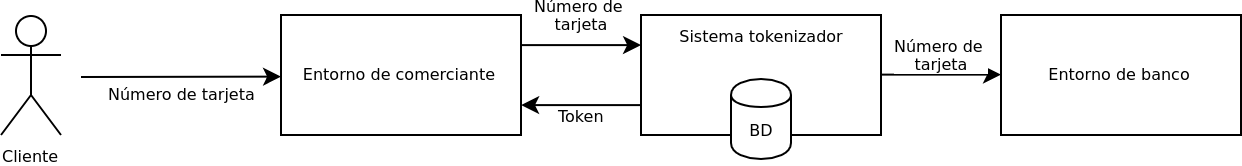
\includegraphics[width=0.8\linewidth]
    {algoritmos_tokenizadores/diagramas/sistema_tokenizador.png}
  \caption{Arquitectura típica de un sistema tokenizador.}
  \label{figura:arquitectura_tokenizacion}
\end{figure*}

% Muestra del problema: ejemplos de discursos publicitarios comunes.

Desde sus inicios, la tokenización se ha visto rodeada por una nube de
desinformación: cada empresa usaba la palabra tokenización sin que existiera una
definición formal, acordada por todos. En 2011, el PCI SSC (\textit{Payment Card
Industry Security Standard Council}) publicó unas guías de tokenización
\cite{pci_tokens} con la idea de ayudar tanto a comerciantes en línea como a
proveedores de servicios de tokenización a esclarecer qué es la tokenización y
qué requerimientos debe de cumplir. Lamentablemente, el PCI no indicó cómo
satisfacer los requerimientos, lo que dio pie a que muchas empresas se siguieran
publicitando como tokenizadoras, sin que los usuarios pudieran saber qué es lo
que pasa adentro de la caja negra.

Una de las consecuencias de esta desinformación es un mensaje bastante común
entre las páginas de las empresas tokenizadoras: la tokenización y la
criptografía son cosas distintas; la tokenización es una alternativa de la
criptografía. Por ejemplo, lo único que \textit{Shift4} dice con claridad sobre
sus tokens es que se trata de valores aleatorios, únicos y alfanuméricos
\cite{shif4_uno} \cite{shif4_dos}; para \textit{Braintree}, la única manera de
generar tokens es por métodos aleatorios \cite{braintree_uno}; para
\textit{Securosis} los tokens son valores aleatorios que nada tienen que ver con
la criptografía \cite{securosis}; \textit{Jack Henry Card Processing Solution},
\textit{Merchant Link} y \textit{Bluepay TokenShield} no mencionan nunca cómo es
que generan sus tokens. La mayoría de las soluciones tratan a sus métodos como
secretos de compañía; esperan que el trato entre cliente y proveedor esté basado
en la confianza y no en la comparación de los propios métodos.

% Establecer relación entre criptografía y tokenización.

Como se verá por la exposición de algunos métodos tokenizadores, la tokenización
es una aplicación de la criptografía y, como tal, debe ser analizada con la
misma formalidad que las demás herramientas criptográficas. Por ejemplo, uno de
los errores más comunes entre las empresas tokenizadoras es considerar a la
generación de números aleatorios como fuera del campo de la criptografía.

% Estructura del artículo.

En la sección dos de este trabajo se tocan algunos temas preliminares necesarios
para presentar, en la sección tres, algunos de los métodos de tokenización. En la
sección cuatro se presentan los resultados de las comparaciones de desempeño
realizadas, y en la sección cinco se concluye con una discusión acerca de las
ventajas y desventajas de cada método.
